\section{Proposed Research}

\subsection{ML Components for Cache and Memory Management}


% Here memory hierarchy is not the whole hierarchy
% TODO Move to intro
%The project will investigate the use of distributed machine leaning components
%from the last-level cache to the main memory, including hardware cache
%prefetching.  Those layers together play a major role in memory system
%performance and energy efficiency. They are also challenging to manage given
%their ever increasing complexity and the diversity of application demands.
%Traditional techniques in cache replacement, cache prefetching, and memory
%access scheduling have been extensively studied, but their gains are increasing
%diminishing.  The recent advance in ML techniques represents a new
%and promising approach to further improve cache and memory performance.

%However, there are unique challenges in applying techniques to optimize the
%cache and memory systems, and more broadly any components inside or partially
%inside a processor.  The ML component must be lightweight and cost-effective;
%otherwise, the performance gain can hardly be justified.  The research on
%performance-oriented NN accelerator, which is the main stream, does not have
%this constraint.  On those accelerator chips, the majority of the chip area is
%dedicated to NN acceleration.  By contrast, a processor chip should only budget
%a small percentage of its chip area for any ML circuits for improving cache and
%memory performance.  Otherwise, the chip area could be used to increase the
%cache capacity.  Additionally, the ML circuits must be energy-efficient.
%High-performance ML accelerator designs, by contrast, tend to be power hungry.

% For large L3 cache, should there be multiple ML components for the
% cache controller?

%Extensive research has been conducted on conventional hardware techniques for
%cache and memory management, including cache organization, multi-level cache
%design, cache replacement policies, cache prefetching, and main memory access
%scheduling.  Those efforts yielded significant results; however, any further
%effort is likely to have diminishing returns.  On the other hand, memory
%performance and memory energy efficiency continue to be a major hurdle for many
%memory-intensive workloads, even with the tremendous advances in cache capacity
%and memory data rates.  They must be complemented by more intelligent management
%techniques.  In fact, the increasing complexity of cache and memory also demands
%further advances in their management.  ML technique is promising in this regard
%because it can explore broader feature spaces for performance correlation.  It
%has been used to improve branch prediction~\cite{} and cache prefetching,
%showing the potential of ML technique to further improve performance on top of
%conventional techniques.  However, the use of ML is limited in scope, and the ML
%circuit design is still primitive.

% ML components should be added to L2 cache controller of each processor core.
% Assume that the processor has 3 levels of cache.

% Cache replacement, cache prefetching, memory access scheduling
% In their decision logic.
% Cache replacement: Affect LRU chain.  It decides by how much a block is prompted.
% What happens to non-LRU design? Pseudo LRU is OK.
% What feedback? If a prompted block is hit, then that's a positive feedback.
%
% One problem is that the feedback unit is expensive, because the past decision
% must be memorized. We can use a general structure for sampled memorization.
% Similar to counting network used in Internet. Each decision is encoded into
% a binary string, and then selectively memorized by sampling. Thus, the resource
% spent on feedback will be fixed.
%
% Any inexpensive feedback unit design?
% Sampling? Bloom filter? Pre-generate positive feedback and negative feedback?
% Cache prefetching: filter prefetching request. Need a feedback unit.
% In the current design (Texas A&M): check if prefetched block is used,
% or rejected block is hit. We need new ideas to show this project's value.
% Memory access scheduling:
%

% Overview

This project will apply ML techniques broadly to the cache and main memory
hierarchy by incorporating distributed and coordinated ML components through the
hierarchy.  It consists of three types of ML components to improve the decision
logic of critical functionalities in the hierarchy, specifically cache
replacement, cache prefetching, and memory access scheduling.  They are embedded
into the corresponding hardware components, namely cache controller, hardware
prefetcher, and memory controller.  They are also connected with each other
using the existing connections among those components, and are coordinated to
improve the learning and inference of each other.

% Discuss why ML components must be efficient at circuit level

% TODO the following paragraph is good, but should be moved to intro

Efficient circuit design for those ML component is critical to this approach,
and will be a major focus of this project.  Unlike ML accelerators used for AI
computing, The circuit of ML components for improving processor performance must
be cost-effective and energy-efficient.  Otherwise, any gains brought by them
may not justify the cost and energy overhead.  They are fundamentally assisting
circuits, not the computing circuits.  By contrast, main-stream ML accelerators
are computing circuits by themselves, and therefore the neural network computing
units can be the major part of the accelerator chips and the energy consumer.
Because of this difference, the ML components for processor performance
improvement must take a different approach than the main stream AI accelerator
design.  The design must be cautious with the circuit cost and energy efficiency
besides prediction accuracy.  Most existing designs in this category use
perceptron-based neural model to avoid expensive multiplication operations, and
uses a relative simple neuron model instead of full neural networks~\cite{}.
One or multiple neurons are constructed dynamically, with the input weights
selected from a set of weight tables using one or multiple feature vectors.  The
neuron outputs will be used to help make a decision, e.g., whether to reject a
prefetch request or which branch target shall be selected.

This proposal uses the same general approach, but explores dynamic feature
selection and weight table design.  It allows a larger feature set than the set
of weight tables, and uses dynamic feature selection to select a set of active
features that actually use the weight tables.  With this new approach, a broad
range of features can be supported with the same cost of weight tables.  Such
cost is typically dozens of kilobytes in existing designs for about a dozen
features.  Thus, a straightforward extension of the feature set is not only
expensive but may significantly increase the energy consumption.  Furthermore,
the weight tables are customized for the selected feature set in the number of
entries and the number of bits per entry.  With dynamic feature selection, the
weight tables need to be more elastic so that they are be used for different
features.

In this approach, dynamic feature selection is critical to the effectiveness of
ML.  An effective feature is one that has high correlation with the prediction
outcome of the ML component.  We will explore several strategy for the dynamic
selection. First, ...

\subsection{The Internal of Cache and Memory MLCs}

\begin{figure}[t]
\centering
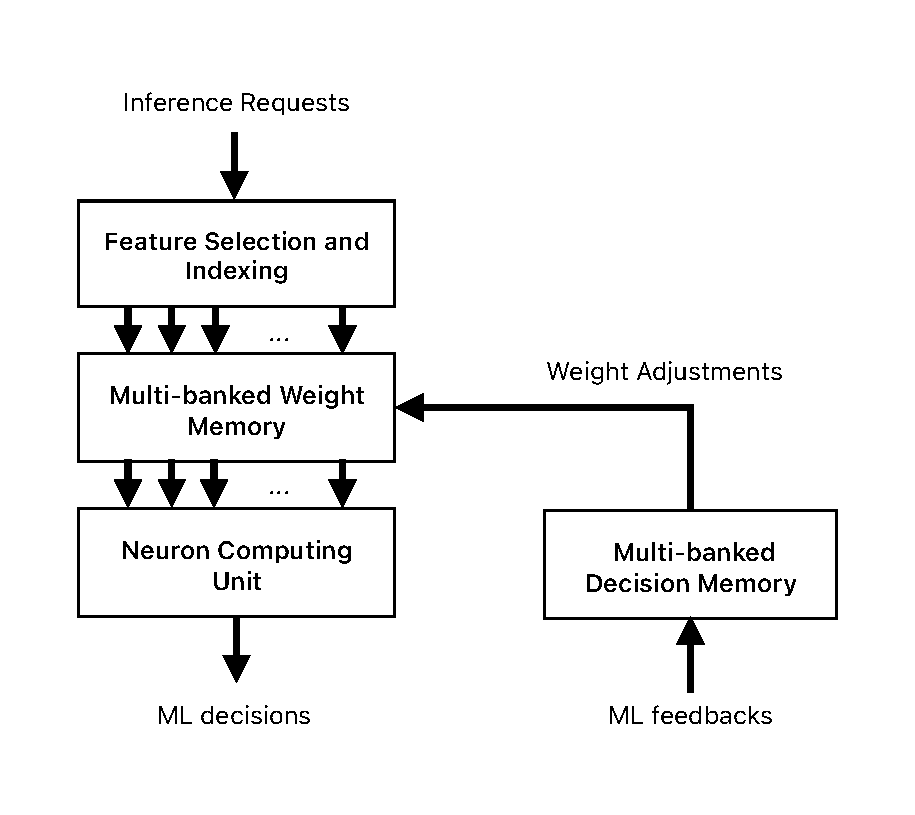
\includegraphics[width=0.8\textwidth]{Figures/ML_Internal.pdf}
\caption{The generic structure of cache and memory MLCs.}
\label{fig:ML-Internal}
\end{figure}

Figure~\ref{fig:ML-Internal} shows the generic internal structure of cache and
memory MLCs.  First of all, cache and memory MLCs rely on online learning, which
is different conventional neural network accelerator design.  The cache and
memory MLCs in this proposal has a key difference from previous designs for
branch prediction and cache prefetching: it uses a multi-banked memory to host
weight tables instead of using separate weight tables.  This is the key to
supporting dynamic feature selection to make the MLCs elastic.  Previous
designs~\cite{} use customized weight tables, where the features, the number of
weight tables, and the number of bits per table entry are all fixed.  The
previous designs have the advantage that, because of the customization, is the
most efficient in circuit implementation. The downside is that it lacks
flexibility: after the processor is fabricated, the feature set is fixed and so
are the circuit details. If the target workloads changes or broadens, the designs
will likely be sub-optimal.

The proposal replaces fully customized weight table with a unified, multi-banked
weight memory, as shown in Figure~\ref{fig:ML-Internal}.  It has multiple access
ports, one per memory bank, and thus can support parallel accesses to weights in
different banks.   With a carefully designed indexing function (see below), it
can serve the same as or close to fully customized tables.  Internally, the
memory banks can be further split sub-banks to for circuit optimizations in
terms of access latency and energy consumption, but the internal structure is
not bound to any feature selection.  Figure~\ref{fig:weight_mem} illustrates the
layout of weight memory to support a given feature set.  The configuration is
done by software, which can use sophisticated algorithms to decide the optimal
layout.

Compared to a fully customized design, unified weight memory is slightly less
efficient for a couple of reasons.  First, the number of bits per weight is now
the same for all features.  Given a particular feature, this parameter could
have been increased for more accuracy or decreased for less energy consumption.
Second, [HERE]

\subsection{ML Component for Cache Replacement}

Cache replacement policy is usually the most important aspect of cache design.
LRU (Least Recently Used) and pseudo LRU policies are commonly used in hardware
cache replacement policies, and they are generally simple and effective.
However, they may perform poorly for certain memory access patterns, e.g., the
scanning of a large data array.  Additionally, they may not explore any
correlation between data reuse and hardware status information, e.g., the PC of
memory instruction, memory page address, the PCs of past memory instructions,
branch history, and so on.  A ML component can explore those correlations to
refine the decision logic of replacement, and thus help improve cache hit rate.

We will explore the integration of ML into the LRU and pseudo-LRU replacement
policies, for which we define a new category named ML-LRU.  In the LRU policy,
all cache blocks form a LRU chain.  On a cache miss, the LRU block, i.e., the
last block in the LRU chain, is replaced, and the new block is placed at the
head of the LRU chain.  On a cache hit, the hit block is moved to the head
position. In ML-LRU, upon a cache hit, the ML component refines the replacement
logic by predicting the best moving distance of the hit block in the LRU chain.
Based on the prediction, a hit block may move to the LRU head position in the
best case, and stay in the same position in the worst case.  Thus, the ML
component may influence the decision logic in cache replacement policy, with
only a minor change of the circuit implementation of the replacement policy.

The ML component may use a number of features that correlate to data reuse
pattern related to the cache block.  It may use the PC of the memory
instruction, which usually has a strong correlation with the data reuse pattern.
In the example of array scanning by a loop, the load instruction alone may
indicate if cache thrashing will happen or not.  If it does, the ML component
may reduce the moving distance in the LRU chain for memory blocks loaded by the
load instruction, which prevents those blocks from replacing other memory blocks
and thus avoids cache thrashing.  In other scenarios, features constructed from
other run-time information may have a strong correlation; for example, memory
page address, branch history, the number of pending memory accesses, and so on.
We will explore those features thoroughly.

[Insert a figure or code]

\subsection{ML Component for Cache Prefetching}

[From Trung's paper]

\subsection{ML Component for Memory Access Scheduling}

Memory access scheduling generally consists of two phases, the ordering of
memory requests and the scheduling of memory operations to serve each
request~\cite{}.  The two phases are distinct but not fully separated.  A good
scheduling scheme may improve memory throughput and energy efficiency.  For
example, the FCFS (First-come First-Serve) policy serves pending memory requests
by their order of arrival, and the FR-FCFS (First-Ready FCFS) policy prioritizes
memory requests that are DRAM row-buffer hits, and then follows the FCFS
policy~\cite{}.  There are more memory access scheduling policies that take into
account memory throughput, bank-level and rank-level parallelism, thread
fairness, and others.

% Discuss the others? PAR-BS, ATLAS, TCM, BLISS.

We will study the integration of an ML component into the memory access
scheduling logic to improve memory throughput and energy efficiency.  Its output
is used to refine the priority of memory requests, which influences the order of
scheduling of memory requests.  The ML component may also influence the decision
to close a row buffer or not, which has significant impact on energy efficiency.
Keeping a memory bank open may significantly improve performance and energy
efficiency if the next access is a row-buffer hit.  Closing a bank, on the other
bank, is the best choice if the next access is a row-buffer miss.  Depending on
the workloads, the optimal decisions of both types can have significant
correlations to load instruction PC, memory page address, memory bus
utilization, row-buffer hit/miss history, request queue length, among others.

The ML component may significantly explore more opportunities than conventional,
rigid schemes, which lacks the flexibility to meet dynamic workload demands.
When combined with a relatively simple scheduling scheme, the new scheme may
achieve the same performance level as each scheme on its target scenarios.  With
a moderate cost, it may provide much more robust performance than conventional
schemes, and explore more opportunities than before.

% I should have discussed the feedback mechanism (learning), but it is tricky.

\subsection{Coordination Framework Through ML Coordinator and Peer
Feedback}

The project further proposes a coordination framework for those ML components in
the cache and memory hierarchy to collaborate with each other.  The coordination
is performed in two forms, namely software coordination and peer feedback.  The
first form is carried out by a new OS kernel module called ML coordinator, which
is executed periodically upon time interrupts and interrupts from ML components.
With the ML coordinator, the ML components may help each other in dynamic
feature selection, as an effective feature at one ML component may also be
effective at another ML component.  We call the first ML component a leader and
the second one a follower.  The software coordinator may read the current
feature selection from special registers of the leader (through memory mapped
I/O) and write to the special registers of the follower so as to transfer
all or part of the feature selection.

This approach allows the software ML coordinator to play an important role in
the coordination, and meanwhile simplifies the hardware interface between the ML
components.  Sophisticated policies and algorithms can be implemented in the ML
coordinator.  For example, if the running workload is a parallel, multithreaded
program, the ML coordinator can proactively synchronize the feature selection of
the ML components associated with those program threads. The ML coordinator may
also periodically evaluate the effectiveness of the coordination, using software
algorithm to decide if the coordination should continue or not.  This approach
is appropriate for dynamic feature selection because the change of feature
selection for a time-consuming program may happen relatively infrequently, e.g.,
at the change of running phases of the current workload.  The overhead of
software-initialized synchronization of the feature selection is relatively low,
and the response time of the software is also acceptable.

Peer feedback provides extra choices of feature input to a ML component from a
peer ML component. For example, a cache MLC may send cache-related features to a
memory MLC; for example, features generated from cache miss rates, cache
utilization rate, active memory regions, and so on.  A memory-MLC may also send
memory-related features to a cache MLC, which may include features generated
from memory bus utilization, bank-level parallelism, read/write queue length,
and so on.  Peer features are selectively enabled like local features.  The
communication utilizes existing wire connections between caches and memory
controllers, and thus they may only cause a negligible increase of the circuit
complexity.

The key questions are how peer features are useful to an MLC, and how to
identify effective peer features to enable.  We believe peer features are useful
additions to local features, because correlation between cache and memory
features are likely to exist between for many workloads.  For example, memory
bus congestion may indicate a change of running phase of the current workload,
which can correlate to the best cache replacement decision in the memory
controller.  The type of correlation may or may not exist, depending on the
workload, running phases, and other factor.  Machine learning is much better
than conventional techniques to explore this opportunity for further performance
improvement, and the use of peer features can enable the exploration.  The
dynamic selection of peer features is similar to that local features, and thus
can rely on the existing mechanism for dynamic feature selection.

% Here there is a question: very high cache miss rate will cause memory bus
% congestion, and thus this feature becomes redundant
%
% There is another issue: peer feedback for learning on peer feature requires
% inter-component communication.  Thus, it means higher energy consumption
% and more congestion.  The feedback has to be infrequent, which may affect
% learning effectiveness.